\def\thudbabelopt{italian}
\documentclass[target=bach,aauheader=,style=]{thud}

\course{Informatica}
\title{Integrazione di Tecnologie Moderne per un CRM Efficiente: Un Caso Studio su Next.js}
\author{Alessandro Gerotto}
\supervisor{Prof.\ Vincenzo Riccio}
\tutor{Yannick Ponte}

\usepackage[a-1b]{pdfx}
\usepackage[pdfa]{hyperref}
\usepackage{multicol}
\usepackage{verbatim}
\usepackage{listings}
\usepackage{xcolor}
\usepackage{graphicx}

\definecolor{lightgray}{rgb}{0.95, 0.95, 0.95}
\definecolor{darkgray}{rgb}{0.4, 0.4, 0.4}
\definecolor{purple}{rgb}{0.65, 0.12, 0.82}
\definecolor{blue}{rgb}{0.0, 0.0, 1.0}
\definecolor{red}{rgb}{1.0, 0.0, 0.0}
\definecolor{green}{rgb}{0.0, 0.5, 0.0}
\definecolor{orange}{rgb}{1.0, 0.5, 0.0}

\lstdefinelanguage{JavaScript}{
  keywords={typeof, new, true, false, catch, function, return, null, switch, var, if, in, while, do, else, case, break, className},
  keywordstyle=\color{orange}\bfseries,
  ndkeywords={class, export, boolean, throw, implements, import, this},
  ndkeywordstyle=\color{blue}\bfseries,
  sensitive=false,
  comment=[l]{//},
  morecomment=[s]{/*}{*/},
  commentstyle=\color{purple}\ttfamily,
  stringstyle=\color{green}\ttfamily,
  morestring=[b]',
  morestring=[b]"
}

\lstdefinelanguage{JavaScriptWithInterface}{
  language=JavaScript,
  morekeywords={id, code, name, startdate, enddate, state, children}, 
  keywordstyle=\color{purple}\bfseries,
}

\lstdefinelanguage{JavaScriptWithTailwind}{
  language=JavaScript,
  morekeywords={main, Navbar, div, Sidebar}, 
  keywordstyle=\color{blue}\bfseries,
}

\lstset{
   language=JavaScript,
   backgroundcolor=\color{lightgray},
   extendedchars=true,
   basicstyle=\footnotesize\ttfamily,
   showstringspaces=false,
   showspaces=false,
   numbers=left,
   numberstyle=\footnotesize,
   numbersep=9pt,
   tabsize=2,
   breaklines=true,
   showtabs=false,
   captionpos=b,
   framerule=0.5pt, % Spessore del riquadro
   rulecolor=\color{darkgray}, % Colore del riquadro
}


\begin{document}
\maketitle
%\begin{dedication}
%	Al mio cane,\par per avermi ascoltato mentre ripassavo le lezioni.
%\end{dedication}

%% Ringraziamenti (opzionali)
%\acknowledgements
%Sed vel lorem a arcu faucibus aliquet eu semper tortor. Aliquam dolor lacus, semper vitae ligula sed, blandit iaculis leo. Nam pharetra lobortis leo nec auctor. Pellentesque habitant morbi tristique senectus et netus et malesuada fames ac turpis egestas. Fusce ac risus pulvinar, congue eros non, interdum metus. Mauris tincidunt neque et aliquam imperdiet. Aenean ac tellus id nibh pellentesque pulvinar ut eu lacus. Proin tempor facilisis tortor, et hendrerit purus commodo laoreet. Quisque sed augue id ligula consectetur adipiscing. Vestibulum libero metus, lacinia ac vestibulum eu, varius non arcu. Nam et gravida velit.

%% Sommario (opzionale)
%\abstract
%Nunc ac dignissim ipsum, quis pulvinar elit. Mauris congue nec leo ornare lobortis. Nulla hendrerit pretium diam nec lobortis. Nullam aliquam laoreet nisl, sit amet facilisis lectus accumsan ut. Duis et elit hendrerit metus venenatis condimentum. Integer id eros molestie, interdum leo sit amet, aliquet metus. Integer fermentum tristique magna, vel luctus neque rhoncus vel. Ut hendrerit et quam et semper. Mauris egestas, odio sed aliquet luctus, magna orci euismod odio, vitae lacinia tellus tellus non lectus. Aliquam urna neque, porta et mattis aliquam, congue sit amet lorem. In ultrices augue sit amet ante vehicula, vitae rhoncus turpis auctor. Donec porta scelerisque eros, at mollis enim imperdiet ut. 

%% Indice
\tableofcontents

%% Lista delle tabelle (se presenti)
%\listoftables

%% Lista delle figure (se presenti)
%\listoffigures

%% Corpo principale del documento
\mainmatter

% Capitolo 1
%\chapter{Introduzione}
%\section{Introduzione Generale}
%\section{Struttura di questa Tesi}

% Capitolo 2
\chapter{Background aziendale}
Archeido \cite{archeido2024} è un'azienda specializzata nell'ingegneria del software, focalizzata sulla creazione e implementazione di soluzioni su architetture cloud-native e infrastrutture Cloud, utilizzando principalmente Amazon Web Services. La missione di Archeido è supportare le aziende durante il processo di trasformazione digitale e adozione del Cloud, offrendo un'assistenza sia tecnica che strategica con massima trasparenza. L'azienda adotta e si basa sulle metodologie DevOps e Agile, garantendo un processo di sviluppo rapido, sicuro ed efficiente.

\section{Prodotto Software}
Il software sviluppato e descritto in questa tesi è un CRM (Customer Relationship Management), progettato per servire come una dashboard centrale per il monitoraggio dei progetti attualmente in corso, come archivio completo di quelli già completati e come piattaforma di pianificazione per i progetti futuri.

\subsection{Funzionalità principali}
Il CRM offre una gestione completa (CRUD) dei progetti, facilitandone le operazioni di creazione, lettura, aggiornamento e cancellazione. Inoltre, consente di monitorare gli utenti autorizzati ad accedere alla dashboard, i quali vengono creati tramite inviti inviati da un super amministratore. A ciascun utente viene assegnato un ruolo specifico, che definisce le regole di visibilità e le autorizzazioni di accesso alle informazioni presenti nella dashboard. Infine, il sistema consente di valutare le performance aziendali, fornendo dati e metriche utili per analizzare l'efficacia dei progetti e il rendimento complessivo del team.

\subsection{Obiettivi del software}
Il CRM ha come obiettivo principale quello di valutare le stime concordate con i clienti, consentendo ai project manager di confrontare le previsioni iniziali stabilite insieme al cliente con i risultati effettivi ottenuti a progetto completato. In questo modo, è possibile identificare eventuali scostamenti e adottare misure correttive tempestive per garantire il successo del progetto. Il CRM sviluppato è dunque uno strumento di monitoraggio che fornisce un supporto strategico volto all'ottimizzazione delle relazioni con i clienti.

\subsection{Stakeholders}
Gli stakeholders di questo progetto includono:

\begin{itemize}
    \item I \textbf{Super Amministratori}, che gestiscono la creazione degli utenti, assegnano loro permessi e regole di visibilitá e hanno accesso completo a tutte le sezioni del CRM. 
    \item I \textbf{Project Manager}, i quali ricevono un account per accedere alla dashboard e possono visualizzare solo i progetti a cui sono stati assegnati, limitando l'accesso ad alcune sezioni.
    \item I \textbf{Clienti}, le cui esigenze influenzano l'uso del CRM, poichè il sistema è progettato per rispondere meglio alle loro necessità.
\end{itemize}

\subsection{Caratteristiche tecniche}
Questo progetto è stato sviluppato utilizzando React e Next.js, sfruttando la libreria NextUI e Tailwind CSS per garantire un'interfaccia utente moderna e responsiva. Next.js \cite{nextjs2024} è ideale per lo sviluppo di applicazioni web grazie al rendering lato server e statico, che ottimizza prestazioni e SEO. La gestione delle route è semplice e la suddivisione automatica del codice accelera i caricamenti.

\section{Ciclo di Vita Adottato}
Archeido adotta un ciclo di vita del software basato su metodologie agili, come Scrum \cite{scrumwiki2024} e Kanban \cite{kanbanwiki2024}, che consentono di gestire progetti in modo iterativo e incrementale. Lo sviluppo Agile si distingue per un approccio meno rigido, focalizzato sull'obiettivo di fornire al cliente software funzionante in tempi brevi e con frequenza. In questo contesto, le fasi di specifica, progettazione, sviluppo, validazione ed evoluzione si susseguono in un processo fluido e non fisso, caratterizzato da una continua negoziazione dei requisiti e raccolta di feedback. L'obiettivo primario è garantire la piena soddisfazione del cliente, andando oltre il semplice adempimento di un contratto.

\section{Problemi e Valutazioni}
Nelle prime fasi dello sviluppo, è stata condotta un'analisi approfondita per valutare quale tra le diverse tecnologie disponibili e librerie grafiche fosse più adatta per la realizzazione del progetto. Alla fine, si è deciso di utilizzare Next.js \cite{nextjs2024} e l'omonima libreria grafica NextUI \cite{nextui2024}. Un altro aspetto cruciale nella fase di sviluppo è stata la scelta tra l'utilizzo di JavaScript puro e l'adozione di TypeScript. Questa decisione ha comportato una valutazione approfondita dei vantaggi e degli svantaggi di entrambe le opzioni, considerando fattori come la tipizzazione statica, la manutenzione del codice e la scalabilità del progetto.

\section{Formazione}
Il primo periodo di questo tirocinio è stato dedicato alla formazione, durante la quale è stata approfondita la programmazione funzionale in JavaScript \cite{knowthen2024}, acquisendo le competenze necessarie per scrivere codice più efficiente e manutenibile. In seguito, si è analizzato React \cite{udemyreactredux2024}, una libreria JavaScript sviluppata da Facebook per la creazione di interfacce utente interattive e componenti riutilizzabili, facilitando lo sviluppo di applicazioni web complesse. Infine, è stato esplorato Next.js, un framework potente che estende le capacità di React, permettendo il rendering lato server e facilitando la creazione di applicazioni web performanti.

% Capitolo 3
\chapter{Background tecnico}

\section{Introduzione}
In questo capitolo, verrà presentato il contesto tecnico del progetto, descrivendo le tecnologie principali utilizzate: TypeScript, React, Next.js, Next UI e Tailwind CSS. Ogni tecnologia verrà analizzata per evidenziarne i punti di forza e come contribuisce alla creazione di un CRM efficace.

\section{JavaScript e TypeScript}
JavaScript \cite{wikipedia:javascript} è un linguaggio di programmazione multi-paradigma, concepito per supportare l'orientamento agli eventi. È utilizzato sia per la programmazione lato client, principalmente nel contesto web, sia per la programmazione lato server, grazie all'uso di Node.js, come approfondito nelle sezioni successive. Tuttavia, nel contesto di questo progetto, si è optato per l'uso di \textbf{TypeScript} \cite{wikipedia:typescript}. Questa scelta è stata effettuata durante la fase iniziale di analisi dei requisiti e il motivo principale è stato che TypeScript ha un \textbf{sistema di tipi statici}. Questo significa che i tipi delle variabili, delle funzioni e delle proprietà vengono definiti al momento della compilazione e non cambiano durante l'esecuzione, permettendo di rilevare gli errori in fase di compilazione piuttosto che durante l'esecuzione. Un altro punto a favore viene evidenziato in contesti dove le applicazioni sono più complesse: TypeScript offre un'architettura di codice più chiara e strutturata. Inoltre, è completamente compatibile con JavaScript, il che consente di integrare senza problemi codice esistente.

\subsection{Le interfacce in TypeScript}
Durante lo sviluppo di questo progetto, si è dimostrata molto utile la definizione a priori di \textbf{interfacce} come linee guida per i modelli dati. Le interfacce fungono da blueprint, definendo i tipi esplicitamente. Al contrario, in JavaScript, la mancanza di un sistema simile rende difficile garantire la conformità a una determinata forma, con errori di tipo che emergono solo durante l'esecuzione.

Ad esempio, per poter creare un nuovo progetto all'interno del CRM, è necessario che esso segua una struttura definita. Attraverso l'uso delle interfacce, è possibile stabilire chiaramente quali proprietà e quali tipi di dati devono essere presenti, garantendo così la corretta integrazione e funzionamento all'interno del sistema.

\begin{lstlisting}[language=JavaScriptWithInterface, caption=Interfaccia di progetto]
    export interface Project {
        id: string;
        code: string;
        name: string;
        startdate: string | number;
        enddate: string | number;
        state: string;
    }
\end{lstlisting}

\section{React}
React è una libreria JavaScript per la creazione di interfacce utente reattive e componenti riutilizzabili. React consente di costruire interfacce utente utilizzando i cosidetti \textbf{componenti} sfruttando \textbf{JSX}, una sintassi di estensione per JavaScript che permette di scrivere codice che combina quest'ultimo con HTML, in un formato che è più leggibile e comprensibile. Nell'esempio qui sotto,  il componente \texttt{Greeting} viene inizializzato usando JavaScript, ma ritorna un codice HTML:

\begin{lstlisting}[caption=Esempio di codice React]
    const name = 'Alice';   
    const Greeting = () => {
        return <h1>Hello, {name}!</h1>
    } 
\end{lstlisting}

\subsection{I componenti}
Un componente React è una funzione JavaScript che rappresenta una parte riutilizzabile e autonoma di un'interfaccia utente in un'applicazione React. I componenti permettono di scomporre l'interfaccia in parti più piccole e gestibili, promuovendo la leggibilitá, la manutenzione e il riuso del codice. Questo approccio basato sui componenti e sulla continua estrazione del codice in componenti piú semplici garantisce diversi vantaggi:

\begin{itemize}
    \item \textbf{Riuso}: Un componente può essere utilizzato in piú parti dell'applicazione, riuducendo la duplicazione del codice.
    \item \textbf{Isolamento}: Ogni componente ha il proprio stato e le proprie proprietà, rendendo il singolo componente utilizzabile e testabile in ambienti isolati, rimuovendone le dipendenze da ció che appare al suo esterno.
    \item \textbf{Composizione di componenti}: Una volta sviluppati diversi componenti, React consente di comporli insieme. Ad esempio, un componente \texttt{Card} potrebbe contenere tre componenti piú semplici: un'immagine, un titolo e un pulsante. Tale Card potrebbe venir poi usata molteplici volte all'interno di un componente piú complesso, come un \texttt{Carousel}.
\end{itemize}

\subsection{Le \textit{props}}
Le props permettono a un componente genitore di fornire informazioni immutabili a un componente figlio, rendendo quest'ultimo più dinamico e flessibile. Un esempio è il seguente:

\begin{minipage}[t]{0.45\textwidth}
    \begin{lstlisting}[caption=Componente genitore]
import React from 'react';
import Greeting from './Greeting';

const App = () => {
    return (
        <div>
            <Greeting name="Alice" />
            <Greeting name="Bob" />
        </div>
    );
};  
    \end{lstlisting}
\end{minipage}
\hfill
\begin{minipage}[t]{0.45\textwidth}
    \begin{lstlisting}[caption=Componente figlio]
import React from 'react';

const Greeting = ({ name }) => {
    return <h1>Hello, {name}!</h1>;
};

export default Greeting;
    \end{lstlisting}
\end{minipage}

In questo esempio, il componente \texttt{Greeting} è una funzione che accetta la prop \texttt{name} e restituisce il testo  "Hello," seguito dal valore della prop \texttt{name}, ottenuta dal componente padre. Per esempio, quando viene passato "Alice" come valore, il risultato renderizzato sarà un'intestazione che dice "Hello, Alice!", mentre se invece viene passato "Bob", verrá stampato "Hello, Bob!".

\section{Next.js}
Next.js \cite{nextjsdocs2024} è un \textit{framework}\footnote{Un insieme di strumenti, librerie e regole che forniscono una struttura di base per lo sviluppo di software, facilitando il lavoro dei programmatori.} React per la creazione di applicazioni web full-stack. Next.js permette di usare i componenti React per costruire interfacce utente, fornendo funzionalità aggiuntive e ottimizzazioni: Next.js astrae e configura automaticamente tutti gli strumenti necessari per React, come il \textit{bundling}, la \textit{compilazione} e il \textit{routing}.

\subsection{Rendering}
Il principale vantaggio di Next.js è l'uso del \textbf{rendering lato server}: i componenti vengono renderizzati direttamente sul server, il cui contenuto viene poi inviato al client. Inoltre, offre la generazione di \textbf{siti statici}, che consente di prerenderizzare determinate pagine e componenti con dati statici durante la costruzione delle applicazioni, rendendoli disponibili al momento del bisogno.

\begin{itemize}
    \item Nel \textbf{Client-Side Rendering (CSR)}, i componenti dell'applicazione vengono raggruppati in un \texttt{bundle} e inviati al client per il rendering. Con l'aumentare della complessità dell'applicazione, la dimensione del \texttt{bundle} cresce, poiché deve includere tutti i componenti necessari. Di conseguenza, un \texttt{bundle} più ampio richiede una quantità maggiore di memoria al client per il caricamento completo. Inoltre, il CSR presenta sfide significative per l'ottimizzazione per i motori di ricerca (SEO) e può esporre dati sensibili contenuti all'interno dei componenti.

    \item Il \textbf{Server-Side Rendering (SSR)} affronta queste problematiche eseguendo il rendering dei componenti direttamente sul server. Tuttavia, i componenti server presentano alcune limitazioni: non possono rispondere a eventi del browser, come clic o modifiche, non possono accedere alle API del browser, non possono mantenere uno stato persistente né utilizzare hook come \texttt{useEffect}.
\end{itemize}

Nelle applicazioni reali, si tende a utilizzare una combinazione di CSR e SSR. L'SSR viene impiegato per la maggior parte delle parti dell'applicazione al fine di ottimizzare i tempi di caricamento, migliorare la SEO e garantire una maggiore sicurezza. Il CSR viene utilizzato solo in situazioni specifiche, per gestire interazioni che richiedono eventi del browser, accesso alle API del browser o gestione dinamica dello stato.

\subsection{App Routing}
Il routing in React gestisce la navigazione tra diverse pagine o componenti all'interno di un'applicazione. Utilizza librerie come \texttt{React Router} per definire percorsi e associare URL specifici a componenti. Quando un utente naviga a un URL, React Router mostra il componente corrispondente senza ricaricare l'intera pagina, permettendo un'esperienza utente fluida e dinamica. In Next.js, il sistema di routing è reso notevolmente più semplice e intuitivo, poiché si basa sulla \textbf{struttura del file system}. Le cartelle rappresentano i percorsi nell'applicazione web, e ogni cartella dedicata a una pagina deve contenere un file chiamato \texttt{page.tsx}\footnote{L'estensione é \texttt{.tsx} perché si sta usando TypeScript. Con JavaScript sarebbe \texttt{.jsx}.}, che include il contenuto della pagina. La cartella \texttt{app} funge da radice del progetto. Ad esempio, nel CRM è stata creata una cartella \texttt{projects}, al cui interno si trova il file \texttt{page.tsx}. In questo file, è stata definita ed esportata una funzione che restituisce un elemento TSX. Questo componente verrà visualizzato quando si visiterà il percorso \texttt{./projects} nella pagina web.

\begin{figure}[htbp]
    \centering
    \vspace{0.8cm} 
    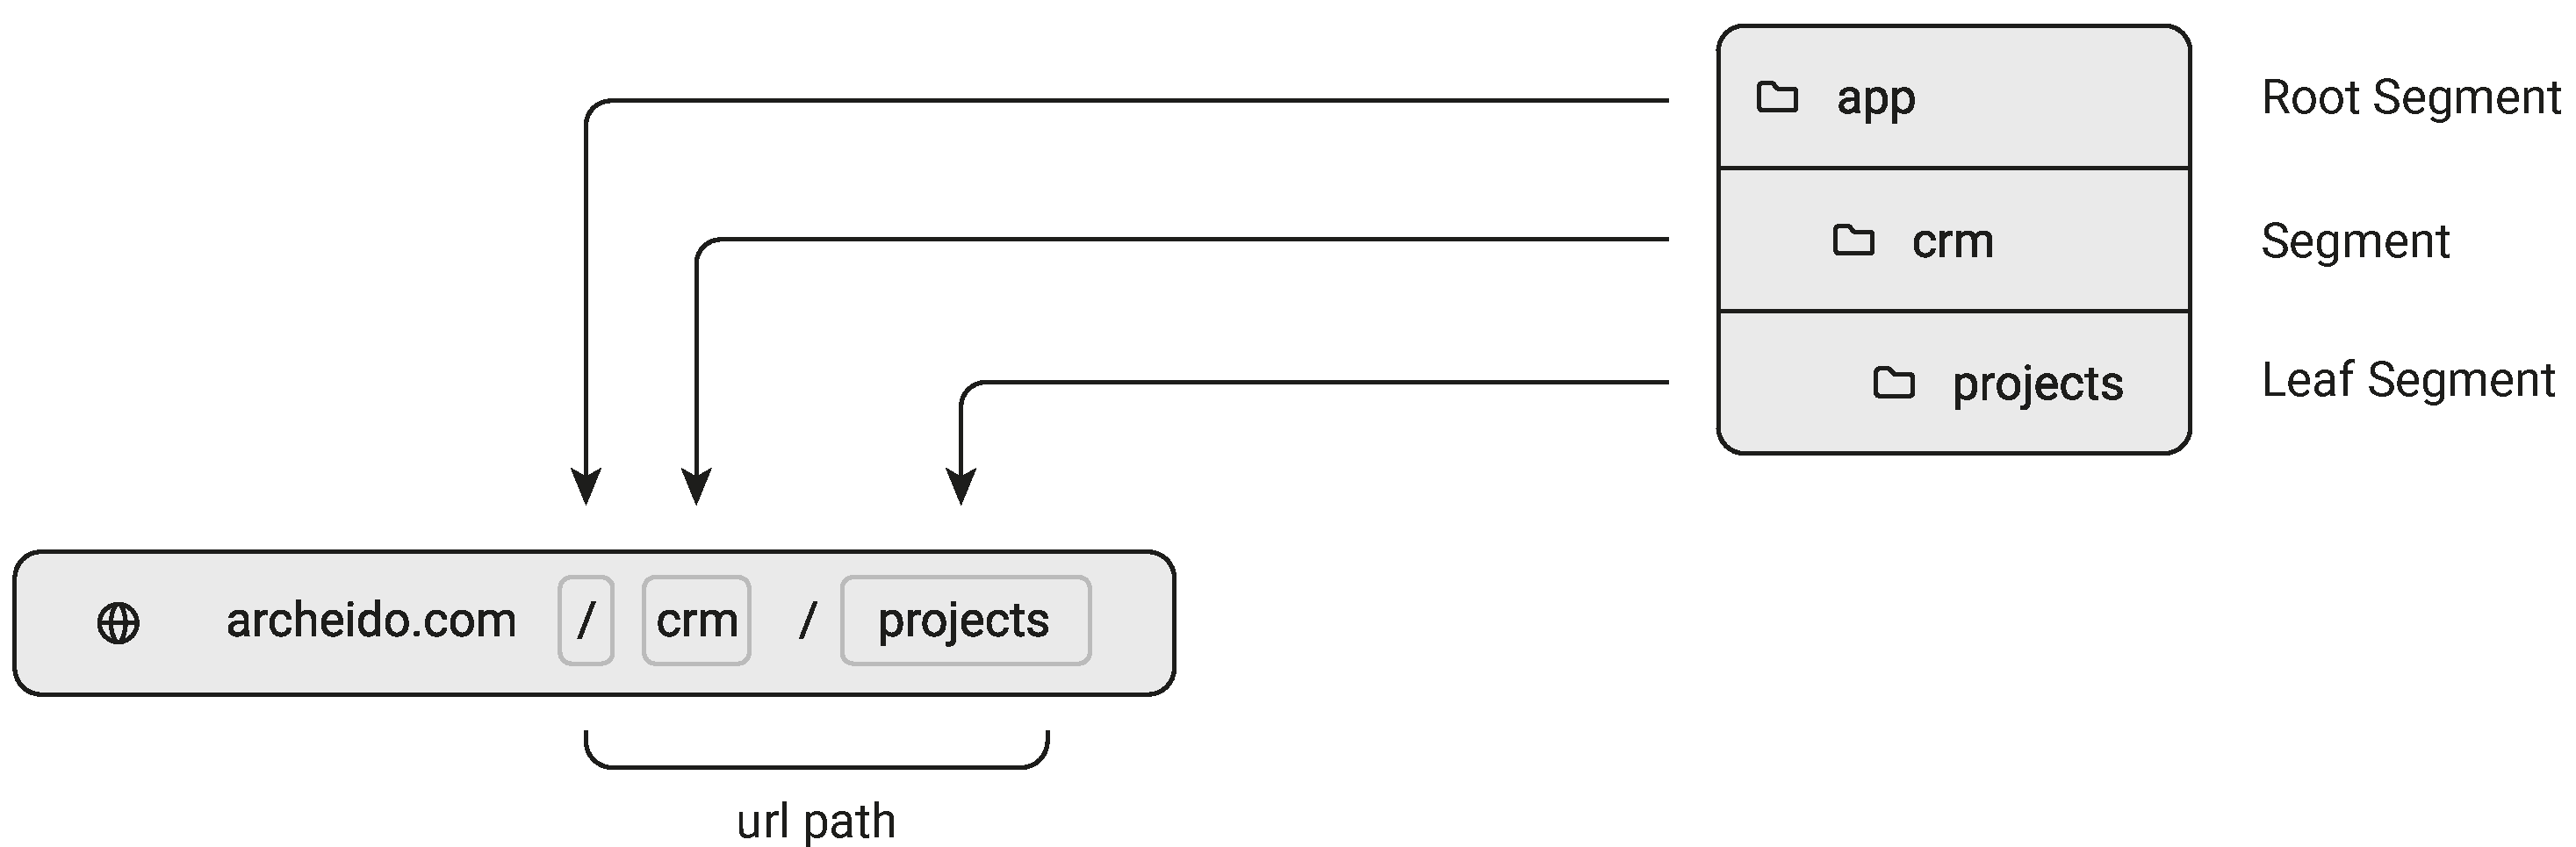
\includegraphics[width=0.9\textwidth]{img/routing.pdf} 
    \caption{App routing \cite{nextjsdocs2024} di Next.js}
    \label{fig:routing} 
\end{figure}



\section{Next UI e Tailwind CSS}
In questo progetto si é deciso di utilizzare Next UI \cite{nextui2024}, la quale è una libreria di componenti UI progettata specificamente per Next.js. Essa offre una serie di componenti predefiniti (come bottoni, modali, cards, chips, etc.) e stilizzati che semplificano la creazione di interfacce utente con un estetica accattivante ma pulita ed intuitiva. 

Un'altra libreria utilizzata per la progettazione del CRM di Archeido é Tailwind CSS: un framework CSS utility-first \footnote{É un approccio alla progettazione di interfacce utente in cui si utilizzano classi CSS per applicare stili direttamente agli elementi HTML, piuttosto che definire classi personalizzate o stili specifici per i componenti.} che permette agli sviluppatori di creare interfacce utente in modo rapido e flessibile. Con Tailwind, é infatti possibile applicare stili direttamente nei file HTML o JSX, rendendo il processo di sviluppo più efficiente. Un esempio é il seguente:
\vspace{0.8cm} 
\begin{lstlisting}[caption=Parte del file \texttt{app.tsx} del CRM]
    <main className="flex flex-col h-screen">
        <Navbar className="w-screen" signOut={signOut} />
        <div className="flex flex-row h-full">
            <div className="col-auto">
                <SideBar />
            </div>
            <div className="col-auto p-8 grow">{children}</div>
        </div>
    </main> 
\end{lstlisting}

%\appendix
%\part{Appendici}
%\chapter{Titolo della prima appendice}

%% Bibliografia
\bibliographystyle{plain_\languagename}
\bibliography{thud}
\end{document}